\section{Bundles, connections, and curvature}
A map out of a higher combinatorial manifold has various components. These line up with classical definitions, and identifying those is a primary purpose of this note.

\subsection{Definitions}

\begin{mydef}
\label{def:connection}
If \( \mm \) is a higher combinatorial \( n \)-manifold and \( f_k:\mm_k\to\uni \) are type families on each skeleton such that all the triangles commute in the diagram:
\end{mydef}
\begin{center}
\chcomment[id=Greg]{Labeled \( \imath_k \)}
% https://q.uiver.app/#q=WzAsNixbMCwwLCJcXG1hdGhiYntNfV8wIl0sWzEsMCwiXFxtYXRoYmJ7TX1fMSJdLFsyLDAsIlxcbWF0aGJie019XzIiXSxbNCwwLCJcXG1hdGhiYntNfSJdLFszLDAsIlxcY2RvdHMiXSxbMiwxLCJcXG1hdGhjYWx7VX0iXSxbMCwxLCJcXGltYXRoXzAiXSxbMSwyLCJcXGltYXRoXzEiXSxbMiw0LCJcXGltYXRoXzIiXSxbNCwzLCJcXGltYXRoX3tuLTF9Il0sWzAsNSwiZl8wIl0sWzEsNSwiZl8xIl0sWzIsNSwiZl8yIl0sWzMsNSwiZiIsMl1d
\begin{tikzcd}
  {\mathbb{M}_0} & {\mathbb{M}_1} & {\mathbb{M}_2} & \cdots & {\mathbb{M}} \\
  && {\mathcal{U}}
  \arrow["{\imath_0}", from=1-1, to=1-2]
  \arrow["{f_0}", from=1-1, to=2-3]
  \arrow["{\imath_1}", from=1-2, to=1-3]
  \arrow["{f_1}", from=1-2, to=2-3]
  \arrow["{\imath_2}", from=1-3, to=1-4]
  \arrow["{f_2}", from=1-3, to=2-3]
  \arrow["{\imath_{n-1}}", from=1-4, to=1-5]
  \arrow["f"', from=1-5, to=2-3]
\end{tikzcd}
\end{center}
and such that for each pushout defining \( \mm_k \) we have the diagram
\begin{center}
% https://q.uiver.app/#q=WzAsNSxbMCwxLCJcXG1hdGhiYntNfV97ay0xfSJdLFswLDAsIk1fa1xcdGltZXMgU15rIl0sWzEsMCwiTV9rIl0sWzEsMSwiXFxtYXRoYmJ7TX1fayJdLFsxLDIsIlxcbWF0aGNhbHtVfSJdLFswLDNdLFsxLDAsIlxccGFydGlhbF97ay0xfSIsMl0sWzIsMywiKl9rIl0sWzEsMiwiXFxtYXRocm17cHJ9XzEiXSxbMywxLCIiLDEseyJzdHlsZSI6eyJuYW1lIjoiY29ybmVyLWludmVyc2UifX1dLFswLDIsImhfayIsMCx7InNob3J0ZW4iOnsic291cmNlIjo0MCwidGFyZ2V0Ijo0MH0sImxldmVsIjoyfV0sWzMsNCwiZl9rIl0sWzAsNCwiZl97ay0xfSIsMl0sWzMsMTIsIiIsMCx7InNob3J0ZW4iOnsidGFyZ2V0IjoyMH19XV0=
\begin{tikzcd}
  {M_k\times S^k} & {M_k} \\
  {\mathbb{M}_{k-1}} & {\mathbb{M}_k} \\
  & {\mathcal{U}}
  \arrow["{\mathrm{pr}_1}", from=1-1, to=1-2]
  \arrow["{\partial_{k-1}}"', from=1-1, to=2-1]
  \arrow["{*_k}", from=1-2, to=2-2]
  \arrow["{h_k}", shorten <=9pt, shorten >=9pt, Rightarrow, from=2-1, to=1-2]
  \arrow[from=2-1, to=2-2]
  \arrow[""{name=0, anchor=center, inner sep=0}, "{f_{k-1}}"', from=2-1, to=3-2]
  \arrow["\ulcorner"{anchor=center, pos=0.125, rotate=180}, draw=none, from=2-2, to=1-1]
  \arrow["{f_k}", from=2-2, to=3-2]
  \arrow[shorten >=2pt, Rightarrow, from=2-2, to=0]
\end{tikzcd}
\end{center}
the outer square of which restricts on each face to the diagram
\begin{center}
\chcomment[id=Greg]{Single-face diagram, outer square}
% https://q.uiver.app/#q=WzAsNCxbMCwxLCJcXG1hdGhiYntNfV97ay0xfSJdLFswLDAsIlxce21fa1xcfVxcdGltZXMgU15rIl0sWzEsMCwibV9rIl0sWzEsMSwiXFxtYXRoY2Fse1V9Il0sWzAsM10sWzEsMCwiXFxwYXJ0aWFsX3trLTF9IiwyXSxbMiwzLCJmX2tcXGNpcmMqX2siXSxbMSwyLCIhIl0sWzAsMiwiXFxmbGF0X2siLDAseyJzaG9ydGVuIjp7InNvdXJjZSI6NDAsInRhcmdldCI6NDB9LCJsZXZlbCI6Mn1dXQ==
\begin{tikzcd}
  {\{m_k\}\times S^k} & {m_k} \\
  {\mathbb{M}_{k-1}} & {\mathcal{U}}
  \arrow["{!}", from=1-1, to=1-2]
  \arrow["{\partial_{k-1}}"', from=1-1, to=2-1]
  \arrow["{f_k\circ*_k}", from=1-2, to=2-2]
  \arrow["{\flat_k}", shorten <=10pt, shorten >=10pt, Rightarrow, from=2-1, to=1-2]
  \arrow[from=2-1, to=2-2]
\end{tikzcd}
\end{center}
then we say
\begin{itemize}
\item The map \( f_k \) is a \defemph{\( k \)-bundle} on \( \mm_k \).
\item The pair given by the map \( f_k \) and the proof \( f_k\circ \imath_{k-1}=f_{k-1} \) that \( f_k \) extends \( f_{k-1} \) is called a \defemph{\( k \)-connection on the bundle \( f_{k-1} \)}.
\item The\chcomment[id=Greg]{diagram permits new wording} filler \( \flat_k \) is called a \defemph{flatness structure for the face \( m_k \)}.
\end{itemize}

The\chcomment[id=Greg]{new lemma} definitions can be digested to give
\begin{mylemma}
Given \( f_{k-1} \) as above, a \( k \)-connection exists if and only if there exists a flatness structure for each \( k \)-face.
\end{mylemma}

\begin{mynote}
Another classical object we can identify here is a \emph{gauge transformation}, which is a bundle automorphism \( H:f\sim f\defeq \pit{m:\mm}f(m)=f(m) \). If we have \( ||H=\id_f||_{-1} \) then the gauge transformation is called \emph{small}, else \emph{large}.
\end{mynote}

\subsection{Connections as local trivializations}
\chcomment[id=Greg]{Capturing our discussion}
This section can ve viewed as an extended remark. The observation we want to make is that the data of a \( k \)-bundle is related to the construction of a trivialization: the fiber at one vertex can be extended throughout the face coherently, using the connection (the extension of the classifying map to the edges) to specify isomorphisms with the fibers at the other points, and the higher connections to establish commutativity between these.

An important context for these remarks is if we imagine that the simplicial complex we started with is in fact a \emph{Cech complex} of a good open cover \( \{U_i\} \) (a cover by contractible open sets, each finite intersection of which is also contractible). This is just to say the vertices \( v_i \) would represent the combinatorial data of the set of charts \( \{U_i\} \) themselves, and the edges are formed if two charts overlap. The \( k \)-faces are the \( k \)-way overlaps, if any. For a good introduction to this point of view, see the introduction in Bott and Tu \cite{bott_tu}. It bears emphasizing: the resulting \emph{higher} types are the same ones we've been working with, it's only the origin of the combinatorial data that we're reimagining.

Continuing the story, the type family \( f \) at one vertex \( v_i \), \( f(v_i) \) would represent a trivial bundle \( U_i\times f(v_i) \) on one chart. Consider a 2-face \( F=\{v_1, v_2, v_3\} \) and types \( f(v_1), f(v_2), f(v_3) \) at the vertices. Extending \( f \) to the edges \( \{e_{12}, e_{23}, e_{31}\} \) provides isomorphisms \( f(e_{12}):f(v_1)=f(v_2) \) and so on. There is a condition to check, however. We need the compatibility \( f(e_{31})\circ f(e_{23})\circ f(e_{12})=\id_{f(v_1)} \) on the 3-way overlap of the charts. This is provided by the flatness structure \( \flat(F) \), which is exactly a proof that the holonomy around the triangle is equal to the identity.\footnote{Not exactly. In Definition~\ref{def:connection} the flatness structure is a homotopy from a hub point to the polygonal boundary. But this is equivalent.}

The classical theory of bundles on smooth manifolds is often presented in terms of just such combinatorial data, constructed from an appropriate atlas of charts and their overlaps. This is very much dual to the viewpoint where points are points, edges are paths, and so on. If one started with a cube, and covered it with six charts that each contained a different face (plus a little overlap), and formed the Cech complex of this data, you would arrive exactly at the dual polyhedron to the cube: the octahedron.

\subsection{The tangent bundle of the sphere}

We will build up a map \( T \) out of \( \oo \) which is meant to be like the circle bundle of a tangent bundle. And so we will begin with the intrinsic data of the link at each point: taking the link of a vertex gives us a map from vertices to polygons.

\begin{mydef}
\( T_0\defeq\link:\oo_0\to\EMzo \) is given by:
\begin{align*}
\link(w) &= brgo & \link(r) &= wbyg \\
\link(y) &= bogr & \link(g) &= wryo \\
\link(b) &= woyr & \link(o) &= wgyb
\end{align*}
We chose these orderings for the vertices in the link, by visualizing standing at the given vertex as if it were the north pole, then looking south and enumerating the link in clockwise order, starting from \( w \) if possible, else \( b \).
\end{mydef}

\begin{figure}[h]
\centering
\begin{figure}[h]
\centering
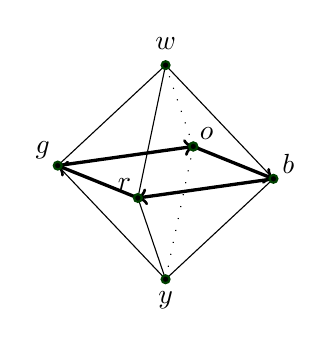
\begin{tikzpicture}%
  [x={(-0.860769cm, -0.121512cm)},
  y={(0.508996cm, -0.205391cm)},
  z={(-0.000053cm, 0.971107cm)},
  scale=1,
  eqback/.style={->, very thick},
  back/.style={loosely dotted, thin},
  eqedge/.style={->, very thick},
  edge/.style={black, thin},
  facet/.style={fill=blue!95!black,fill opacity=0.0},
  vertex/.style={inner sep=1pt,circle,draw=green!25!black,fill=black,thick}]
\coordinate (-1, -1, 0) at (-1, -1, 0);
\coordinate (-1, 1, 0) at (-1, 1, 0);
\coordinate (0, 0, -1) at (0, 0, -1);
\coordinate (0, 0, 1) at (0, 0, 1);
\coordinate (1, -1, 0) at (1, -1, 0);
\coordinate (1, 1, 0) at (1, 1, 0);
%% Drawing edges in the back
%%
\draw[edge,eqback] (-1, -1, 0) -- (-1, 1, 0);
\draw[edge,back] (-1, -1, 0) -- (0, 0, -1.4);
\draw[edge,back] (-1, -1, 0) -- (0, 0, 1.4);
\draw[edge,eqback] (1, -1, 0) -- (-1, -1, 0);
%% Drawing vertices in the back
%%
\node[vertex] at (-1, -1, 0)     {};
%% Drawing the facets
%%
\fill[facet] (1, 1, 0) -- (0, 0, -1.4) -- (1, -1, 0) -- cycle {};
\fill[facet] (1, 1, 0) -- (0, 0, 1.4) -- (1, -1, 0) -- cycle {};
\fill[facet] (1, 1, 0) -- (-1, 1, 0) -- (0, 0, 1.4) -- cycle {};
\fill[facet] (1, 1, 0) -- (-1, 1, 0) -- (0, 0, -1.4) -- cycle {};
%% Drawing edges in the front
%%
\draw[edge] (-1, 1, 0) -- (0, 0, -1.4);
\draw[edge] (-1, 1, 0) -- (0, 0, 1.4);
\draw[eqedge] (-1, 1, 0) -- (1, 1, 0);
\draw[edge] (0, 0, -1.4) -- (1, -1, 0);
\draw[edge] (0, 0, -1.4) -- (1, 1, 0);
\draw[edge] (0, 0, 1.4) -- (1, -1, 0);
\draw[edge] (0, 0, 1.4) -- (1, 1, 0);
\draw[eqedge] (1, 1, 0) -- (1, -1, 0);
%% Drawing the vertices in the front
%%
\begin{scope}[nodes=vertex]
\node[label=above right:\( b \)] at (-1, 1, 0)     {};
\node[label=below:\( y \)] at (0, 0, -1.4)     {};
\node[label=above:\( w \)] at (0, 0, 1.4)     {};
\node[label=above left:\( g \)] at (1, -1, 0)     {};
\node[label=above left:\( r \)] at (1, 1, 0)     {};
\node[label=above right:\( o \)] at (-1, -1, 0)     {};
\end{scope}
\end{tikzpicture}

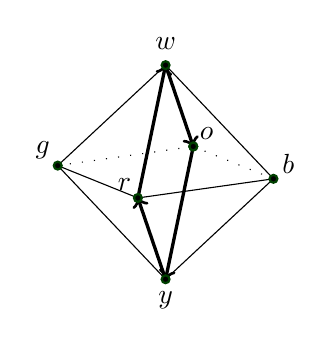
\begin{tikzpicture}%
  [x={(-0.860769cm, -0.121512cm)},
  y={(0.508996cm, -0.205391cm)},
  z={(-0.000053cm, 0.971107cm)},
  scale=1,
  eqback/.style={->, very thick},
  back/.style={loosely dotted, thin},
  eqedge/.style={->, very thick},
  edge/.style={black, thin},
  facet/.style={fill=blue!95!black,fill opacity=0.0},
  vertex/.style={inner sep=1pt,circle,draw=green!25!black,fill=black,thick}]
\coordinate (-1, -1, 0) at (-1, -1, 0);
\coordinate (-1, 1, 0) at (-1, 1, 0);
\coordinate (0, 0, -1) at (0, 0, -1);
\coordinate (0, 0, 1) at (0, 0, 1);
\coordinate (1, -1, 0) at (1, -1, 0);
\coordinate (1, 1, 0) at (1, 1, 0);
%% Drawing edges in the back
%%
\draw[edge,back] (-1, -1, 0) -- (-1, 1, 0);
\draw[edge,eqback] (-1, -1, 0) -- (0, 0, -1.4);
\draw[edge,eqback] (0, 0, 1.4) -- (-1, -1, 0);
\draw[edge,back] (1, -1, 0) -- (-1, -1, 0);
%% Drawing vertices in the back
%%
\node[vertex] at (-1, -1, 0)     {};
%% Drawing the facets
%%
\fill[facet] (1, 1, 0) -- (0, 0, -1.4) -- (1, -1, 0) -- cycle {};
\fill[facet] (1, 1, 0) -- (0, 0, 1.4) -- (1, -1, 0) -- cycle {};
\fill[facet] (1, 1, 0) -- (-1, 1, 0) -- (0, 0, 1.4) -- cycle {};
\fill[facet] (1, 1, 0) -- (-1, 1, 0) -- (0, 0, -1.4) -- cycle {};
%% Drawing edges in the front
%%
\draw[edge] (-1, 1, 0) -- (0, 0, -1.4);
\draw[edge] (-1, 1, 0) -- (0, 0, 1.4);
\draw[edge] (-1, 1, 0) -- (1, 1, 0);
\draw[edge] (0, 0, -1.4) -- (1, -1, 0);
\draw[eqedge] (0, 0, -1.4) -- (1, 1, 0);
\draw[edge] (0, 0, 1.4) -- (1, -1, 0);
\draw[eqedge] (1, 1, 0) -- (0, 0, 1.4) ;
\draw[edge] (1, 1, 0) -- (1, -1, 0);
%% Drawing the vertices in the front
%%
\begin{scope}[nodes=vertex]
\node[label=above right:\( b \)] at (-1, 1, 0)     {};
\node[label=below:\( y \)] at (0, 0, -1.4)     {};
\node[label=above:\( w \)] at (0, 0, 1.4)     {};
\node[label=above left:\( g \)] at (1, -1, 0)     {};
\node[label=above left:\( r \)] at (1, 1, 0)     {};
\node[label=above right:\( o \)] at (-1, -1, 0)     {};
\end{scope}
\end{tikzpicture}

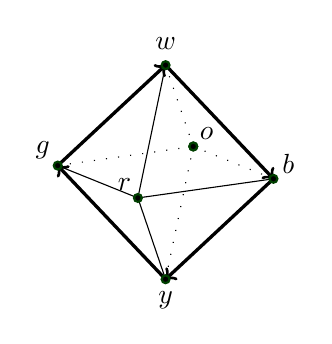
\begin{tikzpicture}%
  [x={(-0.860769cm, -0.121512cm)},
  y={(0.508996cm, -0.205391cm)},
  z={(-0.000053cm, 0.971107cm)},
  scale=1,
  eqback/.style={->, very thick},
  back/.style={loosely dotted, thin},
  eqedge/.style={->, very thick},
  edge/.style={black, thin},
  facet/.style={fill=blue!95!black,fill opacity=0.0},
  vertex/.style={inner sep=1pt,circle,draw=green!25!black,fill=black,thick}]
\coordinate (-1, -1, 0) at (-1, -1, 0);
\coordinate (-1, 1, 0) at (-1, 1, 0);
\coordinate (0, 0, -1) at (0, 0, -1);
\coordinate (0, 0, 1) at (0, 0, 1);
\coordinate (1, -1, 0) at (1, -1, 0);
\coordinate (1, 1, 0) at (1, 1, 0);
%% Drawing edges in the back
%%
\draw[edge,back] (-1, -1, 0) -- (-1, 1, 0);
\draw[edge,back] (-1, -1, 0) -- (0, 0, -1.4);
\draw[edge,back] (-1, -1, 0) -- (0, 0, 1.4);
\draw[edge,back] (1, -1, 0) -- (-1, -1, 0);
%% Drawing vertices in the back
%%
\node[vertex] at (-1, -1, 0)     {};
%% Drawing the facets
%%
\fill[facet] (1, 1, 0) -- (0, 0, -1.4) -- (1, -1, 0) -- cycle {};
\fill[facet] (1, 1, 0) -- (0, 0, 1.4) -- (1, -1, 0) -- cycle {};
\fill[facet] (1, 1, 0) -- (-1, 1, 0) -- (0, 0, 1.4) -- cycle {};
\fill[facet] (1, 1, 0) -- (-1, 1, 0) -- (0, 0, -1.4) -- cycle {};
%% Drawing edges in the front
%%
\draw[eqedge] (-1, 1, 0) -- (0, 0, -1.4);
\draw[eqedge] (0, 0, 1.4) -- (-1, 1, 0);
\draw[edge] (-1, 1, 0) -- (1, 1, 0);
\draw[eqedge] (0, 0, -1.4) -- (1, -1, 0);
\draw[edge] (0, 0, -1.4) -- (1, 1, 0);
\draw[eqedge] (1, -1, 0) -- (0, 0, 1.4);
\draw[edge] (0, 0, 1.4) -- (1, 1, 0);
\draw[edge] (1, 1, 0) -- (1, -1, 0);
%% Drawing the vertices in the front
%%
\begin{scope}[nodes=vertex]
\node[label=above right:\( b \)] at (-1, 1, 0)     {};
\node[label=below:\( y \)] at (0, 0, -1.4)     {};
\node[label=above:\( w \)] at (0, 0, 1.4)     {};
\node[label=above left:\( g \)] at (1, -1, 0)     {};
\node[label=above left:\( r \)] at (1, 1, 0)     {};
\node[label=above right:\( o \)] at (-1, -1, 0)     {};
\end{scope}
\end{tikzpicture}
\caption{The equators for \( w, b, r \).}
\end{figure}
\caption{\( \link \) for the vertices \( w, b\) and \( r \).}
\label{fig:triangle_of_equators}
\end{figure}

To extend \( T_0 \) to a function \( T_1 \) on the 1-skeleton we have complete freedom. Defining a map by induction makes clear that the action on paths is its own structure. Two functions on the octahedron could agree on points but differ on edges. We are going to identify this 1-dimensional freedom with a connection:

Continuing the example, we will do something ``tangent bundley'', imagining how \( T_1 \) changes as we slide from point to point in the embedding shown in the figures. Sliding from \( w \) to \( b \) and tipping the link as we go, we see \( r\mapsto r \) and \( o\mapsto o \) because those lie on the axis of rotation. Then \( g\mapsto w \) and \( b\mapsto y \). 

\begin{mydef}
Define \( T_1:\oo_1\to\EMzo \) on just the 1-skeleton by extending \( T_0 \) as follows:
Transport away from \( w \):
\begin{itemize}
\item \( T_1(wb):[b, r, g, o]\mapsto [y, r, w, o] \) (\( r, o \) fixed)
\item \( T_1(wr):[b, r, g, o]\mapsto [b, y, g, w] \) (\( b, g \) fixed)
\item \( T_1(wg):[b, r, g, o]\mapsto [w, r, y, o] \)
\item \( T_1(wo):[b, r, g, o]\mapsto [b, w, g, y] \)
\end{itemize}
Transport away from \( y \):
\begin{itemize}
\item \( T_1(yb):[b, o, g, r]\mapsto [w, o, y, r] \)
\item \( T_1(yr):[b, o, g, r]\mapsto [b, y, g, w] \)
\item \( T_1(yg):[b, o, g, r]\mapsto [y, o, w, r] \)
\item \( T_1(yo):[b, o, g, r]\mapsto [b, w, g, y] \)
\end{itemize}
Transport along the equator:
\begin{itemize}
\item \( T_1(br):[w, o, y, r]\mapsto [w, b, y, g] \) 
\item \( T_1(rg):[w, b, y, g]\mapsto [w, r, y, o] \)
\item \( T_1(go):[w, r, y, o]\mapsto [w, g, y, b] \)
\item \( T_1(ob):[w, g, y, b]\mapsto [w, o, y, r] \)
\end{itemize}
\end{mydef}

It's very important to be able to visualize what \( T_1 \) does to triangular paths such as \( wb\cdot br\cdot rw \) (which circulates around the boundary of face \( wbr \)). You can see it if you imagine Figure~\ref{fig:triangle_of_equators} as the frames of a short movie. Or you can place your palm over the top of a cube and note where your fingers are pointing, then slide your hand to an equatorial face, then along the equator, then back to the top. The answer is: you come back rotated clockwise by a quarter-turn. 

\begin{mydef}
\label{def:octahedron_holonomy}
The map \( R:C_4\to C_4 \) rotates by one quarter turn, one ``click":
\begin{multicols}{2}
\begin{itemize}
\item \( R(c_1) = c_2 \)
\item \( R(c_2) = c_3 \)
\item \( R(c_3) = c_4 \)
\item \( R(c_4) = c_1 \)
\item \( R(c_1c_2) = c_2c_3 \)
\item \( R(c_2c_3) = c_3c_4 \)
\item \( R(c_3c_4) = c_4c_1 \)
\item \( R(c_4c_1) = c_1c_2 \)
\end{itemize}
\end{multicols}
\end{mydef}

Note by univalence the equivalence \( R \) gives a loop in the universe, a term of \( C_4=_{\EMzo}C_4 \).

Now let's extend \( T_1 \) to all of \( \oo \) by providing values for the eight faces. The face \( wbr \) is a path from \( \refl_w \) to the concatenation \( wb\cdot br\cdot rw \), and so the image of \( wbr \) under the extended version of \( T_1 \) must be a homotopy from \( \refl_{T_1(w)} \) to \( T_1(wb\cdot br\cdot rw) \). Here \emph{there is no additional freedom}.

\begin{mydef}
\label{def:octahedron_curvature}
Define \( T_2:\oo\to\EMzo \) by extending \( T_1 \) to the faces as follows:
\begin{multicols}{2}
\begin{itemize}
\item \( T_2(wbr)=H_R \) 
\item \( T_2(wrg)=H_R \)
\item \( T_2(wgo)=H_R \)
\item \( T_2(ybo)=H_R \)
\item \( T_2(yrb)=H_R \) 
\item \( T_2(ygr)=H_R \)
\item \( T_2(yog)=H_R \)
\item \( T_2(ybo)=H_R \)
\end{itemize}
\end{multicols}
where \( H_R:R=\refl_{C_4} \) is the obvious homotopy given by composition with \( R^{-1} \). Passing through univalence we get a 2-path between \( R \) and \( \refl \) in the loop space \( C_4=_{\EMzo}C_4 \).
\end{mydef}

\subsection{Existence of connections}

How confident can we be that we can always define a connection on an arbitrary combinatorial manifold? Two things make the octahedron example special: the link is a 4-gon at every vertex, and every edge extends to a symmetry of the entire octahedron, embedded in 3-dimensional space. This imposed a coherence on the interactions of all the choices we made for the connection, which we can worry may not exist for more complex combinatorial data.

We know as a fact outside of HoTT that any combinatorial surface that has been realized as a triangulated surface embedded in 3-dimensional euclidean space can inherit the parallel transport entailed in the embedding. We could then approximate that data to arbitrary precision with enough subdivision of the fibers of \( T \).

What would a proof inside of HoTT look like? We will leave this as an open question.

